\section{Method}
\label{sec:method}

The main focus of this study is on the data and evaluation. We thus
keep the components of our architecture simple, and follow established
modeling practices whenever possible.

\subsection{Dataset}
We use the dataset provided by \citet{papasarantopoulos2021narration}
containing a metadata for the set of 209 episodes (seasons 1--5) of the
English-language version of {\it Peppa Pig}. We purchased the
corresponding Peppa Pig episodes in the form of DVDs. 

These annotations created by  \citet{papasarantopoulos2021narration}
feature written transcriptions aligned with the
audio as well as segmentation into {\it dialog} and {\it
  narration}.\footnote{It should be noted that the quality of the
  alignment and segmentation in the original dataset is variable. In
  cases where exact alignment is needed, such as for word-level
  analyses, we re-align the transcriptions using
  \url{github.com/lowerquality/gentle}.}  Dialogs are the parts spoken
by the characters, while narrations are comments inserted by the
narrator, which are more descriptive in nature. All the narration
segments are uttered by the same voice actor. We use the dialogs for
training the model, and set aside the narrations for evaluation
purposes only. A small portion of the dialog data is also used for
validation.  Specifically, out of the total 209 episodes, we use
dialog from episodes 1--196 for training, and 197--209 for
validation. We set aside narrations from episodes 1--104 for
validation and 105--209 for testing. \Cref{tab:ds-stat}
shows the sizes of the training and validation splits.

\begin{table}[htb]
  \centering \begin{tabular}{llrr}
	\toprule
	Split &      Type &  Size (h) &  \# Clips \\
	\midrule
	train &    dialog &     10.01 &    15666 \\
	val &    dialog &      0.66 &     1026 \\
	val & narration &      0.94 &     1467 \\
	test & narration &      0.64 &     1006 \\
	\bottomrule
\end{tabular}

  \caption{Duration in hours of the dataset splits.}
  \label{tab:ds-stat}
\end{table}


\subsection{Preprocessing}
Our model is trained to discriminate positive video-audio pairs from
negative ones.  The positive pairs are those that are temporally
coincident in the original video file. In order to generate these
training items we need to split the videos into fragments.  For
segmenting data for training, we \emph{do not} use word or
sentence-level subtitle alignment in order to make the setting
naturalistic. Processing long segments of video and audio is not
tractable on commodity GPU hardware, and we thus segment the data into
brief snippets roughly comparable in length to the duration a short
sentence or a phrase. We use the following two segmentation
strategies:

\paragraph{Fixed} Using this approach we simply split sections into
fixed-length non-overlapping fragments of 2.3 second duration. This
length is close to the mean duration of audio aligned to a single line
of subtitles.

\paragraph{Jitter} In this approach the mean duration of the segments
is the same (2.3 seconds) but we randomly vary the length of the
video, and independently, of the corresponding audio around this
average duration. This means that (i) the segments can be partially
overlapping and (ii) the video and the audio it is paired with are
normally of different length. Specifically we sample the fragment
duration $d$ (in seconds)
from the following distribution:
\begin{equation}
  d \sim \min(6, \max(0.05, \mathcal{N}(2.3, 0.5)))
  \label{eq:jitter}
\end{equation}
The video is subsampled to 10 frames per second, and to
$180\times 100$ resolution.\footnote{Performance is better with higher
  resolution (we tried $360\times 200$), but it makes GPU memory
  requirements prohibitive.}  The audio is converted to mono by
averaging the two channels and the raw waveform is used as input. We
use the original sample rate of 44.1 kHz (instead of downsampling to
the 16 kHz sample rate used for pre-training \textsc{wav2vec2}) as we
found out that this helps with generalization performance on the
narration validation data.

For evaluation we have a number of different conditions and evaluation
metrics described in detail in \Cref{sec:eval} and in some of these
conditions we use the subtitles to guide
segmentation. 



\subsection{Model Architecture}
\label{sec:model}
We adapt the high-level modeling approach from work on spoken
image-caption data
\citep{harwath2016unsupervised,chrupala-etal-2017-representations}:
our objective function is based on a triplet-like contrastive loss with margin which
encourages the matching audio and video clip to be projected nearby in
the embedding space, and mis-matching audio and video clips to be far
away:
\begin{dmath}
  \ell = \sum_{av}\left[\sum_{a'} \max(0, S_{a'v} - S_{av} +
    \alpha) + \sum_{v'} \max(0, S_{av'} - S_{av} + \alpha) \right]
  \label{eq:triplet}
\end{dmath}
where $\alpha$ is a margin, $S_{av}$ is a similarity score between a
matching audio-video clip pair, and $S_{a'v}$ and $S_{av'}$ denote
similarity scores between mismatched pairs, i.e.\ negative examples
from the current batch. Our heuristic to generate positive and
negative examples is very simple: we consider the example
positive if the audio is aligned with a video clip in our
data. Other pairs of audio-video clips are considered negative.

\subsubsection{Audio Encoder}
The audio encoder portion of the model consists of a {\tt small
  wav2vec2} model \citep{wav2vec2} pre-trained in a self-supervised
fashion, without any supervised fine tuning.\footnote{Available from
  \url{https://dl.fbaipublicfiles.com/fairseq/wav2vec/wav2vec_small.pt}.}
The \textsc{wav2vec 2.0} architecture learns audio embeddings by
self-supervised learning driven by a contrastive loss applied to 
quantized latent representations of masked frames, loosely inspired by
the BERT approach to language modeling \citep{devlin-etal-2019-bert}.

The output of this module is a temporal sequence of 28-dimensional vectors. We
pool this output across time using an attention mechanism with
dimension-wise weights \citep{Merkx2019}:
\begin{equation}
  \begin{aligned}
    \mathbf{A} = & \mathrm{softmax}_t\left(\mathrm{MLP}(\mathbf{X})\right)\\
    \mathbf{z} = & \sum_t \left( \mathbf{A}_{t} \odot \mathbf{X}_{t} \right),
  \end{aligned}
  \label{eq:att-pool}
\end{equation}
where $\mathbf{X}$ is the tensor with the encoder output vectors for
each time-step $t$: an MLP followed by a time-wise
softmax is used to compute an attention weight for each time step and for each
dimension.
%Each dimension of the pooled embedding vector $\mathbf{z}$
%consists of a weighted sum across time of the output values at this
%dimension.
The pooling is followed by a linear projection and $L_2$
normalization. For our experiments we also use versions of the encoder
where the wav2vec weights are frozen, as well a randomly initialized
rather than pre-trained.



\subsubsection{Video Encoder}
As a video encoder we use the 18-layer ResNet (2+1)D architecture
\citep{tran2018closer} pretrained on the action recognition dataset
Kinetics-400 \citep{DBLP:journals/corr/KayCSZHVVGBNSZ17}. The
pre-trained model is available via Pytorch.\footnote{See
  \url{https://pytorch.org/vision/0.8/models.html\#resnet-3d}.}  This
architecture implements 3D convolution by decomposing it into a 2D
spatial convolution followed by 1D temporal convolution.  The output
of this module is aggregated using the attention mechanism with the
same architecture as for the audio module, linearly projected to the
same dimensionality as the audio (512) and $L_2$ normalized.  For our
experiments we also use a version of the video encoder without
pre-training.

\paragraph{\textsc{Static} baseline}
As a baseline to investigate the contribution of temporal information to
video modeling we swap the video ResNet (2+1)D with the D2 ResNet
pre-trained on ImageNet, which embeds each video frame
separately. These frame embeddings are then attention-pooled as with
the standard video encoder. 


\subsection{Evaluation}
\label{sec:eval}
The most common approach to evaluation for visually grounded models
trained on spoken image captions is caption-to-image retrieval (often
combined with image-to-caption retrieval): in fact this technique
has been carried over from text-based image-caption modeling.
 With the standard spoken caption dataset this approach is unproblematic since
the content of the captions is not correlated with extra-linguistic
clues in the speech signal, such as speaker identity (since speakers
are randomly assigned to captions) or non-speech environmental
sounds. In such an artificial setting, a retrieval metric measures the ability of the
model to match spoken utterances to images based on their semantic
content. This is not the case for the {\it Peppa Pig} dataset: here we
can expect that when a video segment depicts a particular character
(e.g.\ George) then the audio in this segment is more likely to contain
utterances spoken by the voice actor playing George.  Moreover, some 
characters might have a tendency to talk about certain topics more often 
than others, and the model might pick up on these associations instead of 
paying attention to the actual meaning of the uttered words.
%
%George has a
%favorite toy dinosaur: when this toy appears in a video segment we can
%likewise expect higher than random chance of George's voice in the
%audio. 
Due to these factors, in a naive retrieval setting, a model
could obtain a high score by mostly capturing these non-linguistic
correlations.

In order to control for these factors we leverage the
narrator speech in the videos. These utterances are always spoken by
the same actor, so speaker identity cannot be used as a clue for
matching video and audio. Furthermore, the narration segments are akin
to video captions in that they tend to describe what is happening in
the video and thus their semantic content is more strongly
correlated with the content of the video than in the case of the
dialog, which is also a desirable feature for the purposes of system
evaluation.

To further investigate the contributions of temporal information in the 
videos, we additionally evaluate model performance in a condition where we 
randomly scramble the video frames within a clip at test time, thereby removing 
any useful temporal information.

\subsubsection{Video Retrieval}
\label{sec:retrieval}
For the retrieval evaluation, as for training, we use the
\textsc{fixed} and \textsc{jitter} segmentation strategies. We encode
each audio clip in a candidate set sampled from the validation (or
test) data using the speech encoder part of the model; we encode each
video clip using the video encoder. We then measure cosine similarity
between the audio clip and all the video clips. If the video clip
corresponding to the audio is among the $n$ most similar video clips,
we count that as a success. The proportion of successes across all
audio clips gives us the retrieval metric known as recall@$n$:
specifically in this paper we focus on $n=10$. We set the candidate
set size to $100$, and thus the random baseline for the recall@10 is
$10$\%. In order to quantify uncertainty in this evaluation due to the
test data we repeat this procedure 500 times with randomly sampled
candidate sets and visualize the score distribution.  


\subsubsection{Triplets}
\label{sec:triplets}
Retrieval metrics such as recall@10 have some disadvantages. Firstly
the absolute value of this metric may be hard to interpret as it depends
on the size of the candidate set. Secondly, if
we wanted to compare model performance with human performance, we
could not feasibly ask human participants to provide the quadratic
number of audio-video similarity judgments needed. For these reasons,
we evaluate model performance using a more simple and controlled scenario, 
inspired by intermodal preferential looking paradigms in child
language acquisition \citep{hirsh1996intermodal}.


\begin{figure}
	\centering
	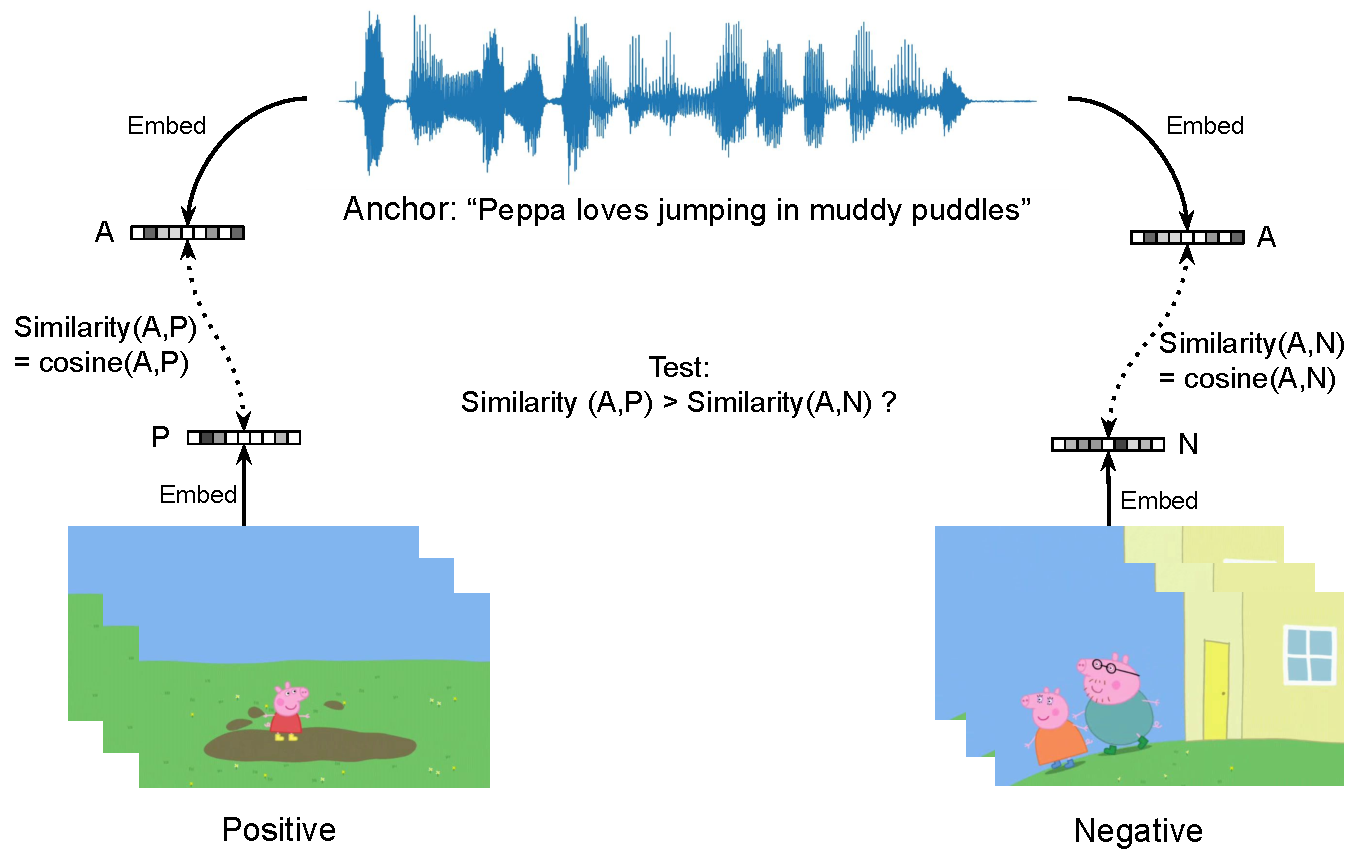
\includegraphics[width=\columnwidth]{peppa_triplets_eval_detailed.pdf}
	\caption{Triplets Evaluation: Given a reference audio sequence (anchor), we 
	measure the model's performance at choosing the matching video (positive) 
	over a random distractor video (negative).}
	\label{fig:triplets_eval}
\end{figure}

We extract clips aligned to a single subtitle
line, group them by length, and for each pair of same-length video
clips\footnote{To keep test items independent, the pairing of video
  clips is done such that each clip only occurs as a member of a single
  triplet.}, we extract the audio from one of them (selected at
random) -- this is our {\it anchor}. The video clip from which the
anchor was taken is the {\it positive} one, which the other video clip
is the {\it negative} one. This triplet of stimuli form a single test
item.  We use the model's audio encoder to encode the anchor, and the
video encoder to encode both video clips. We then check whether anchor
is more similar to the positive or negative clips in terms of cosine
similarity (see also \Cref{fig:triplets_eval}).  More precisely, {\it triplet 
accuracy} is the mean over
all triplets of the following quantity:
\begin{equation}
  \frac{\mathrm{signum}(\mathrm{cosine}(A, P) - \mathrm{cosine}(A, N)) + 1}{2}
  \label{eq:triplet-acc}
\end{equation}
with $A$ being the anchor, $P$ positive and $N$ negative. The triplet
accracy metric is inspired by the ABX score of \citet{schatz2016abx}. \todo{MN: 
that might be confusing for the reader: we first say it's inspired by 
preferential looking and then by ABX score. Maybe we can only say once that's 
inspired by the two of them?}
For triplet accuracy, regardless of the specific set of test items, we
expect random-guessing performance to be at 0.5, and perfect
performance to be 1.0. For this metric we also quantify uncertainty by
resampling the triplets $500$ times from the dataset, and display the
score distribution.

\subsubsection{Minimal Pairs}
\label{sec:targeted}
While the triplet evaluation gives us a general idea about whether the model 
has learned a mapping between videos and audio, the metric does not provide 
insight into whether the model has acquired the grounded semantics of specific 
words.

To address this question, we probe the model's performance in a more targeted 
triplet setup, where the model is required to select the correct video from a 
pair of videos with \textit{minimal differences} regarding a target word in the 
corresponding transcripts.
We pair every triplet with a corresponding counter-example to 
control the evaluation for linguistic biases in the dataset \citep[see 
also][]{nikolaus-fourtassi-2021-evaluating}.
%and thereby ensure that a single-modality model that only considers the audio 
%performs at chance 

To construct the evaluation set, we search the transcripts of the validation 
data for phrases with minimal differences with respect to the most commonly 
occurring (at least 10 times) nouns, verbs, and adjectives. We set the minimum 
phrase duration to 0.3 seconds.\footnote{For shorter sequences, we do not 
expect that the video contains enough semantic information to 
distinguish target and distractor. A phrase can also be a single word.}

Based on the video and audio of each pair of phrases, we create two 
counter-balanced test trials (example and counter-example), as depicted in
\Cref{fig:minimal_pairs}. Here, the anchor $A_{\text{example}}$ of the example
triplet is the audio of \textit{Peppa loves jumping}, the positive video 
$P_{\text{example}}$ is the corresponding video, and the negative video 
$N_{\text{example}}$ is the video corresponding to \textit{George loves 
jumping}. In the counter-example triplet, the anchor $A_{\text{counterex}}$ is 
the audio of \textit{George loves jumping}, and the positive and negative video 
are flipped. % $P_{\text{counterex}} = N_{\text{example}}; N_{\text{counterex}} 
%= P_{\text{example}}$.

\begin{figure}[ht]
  \centering
  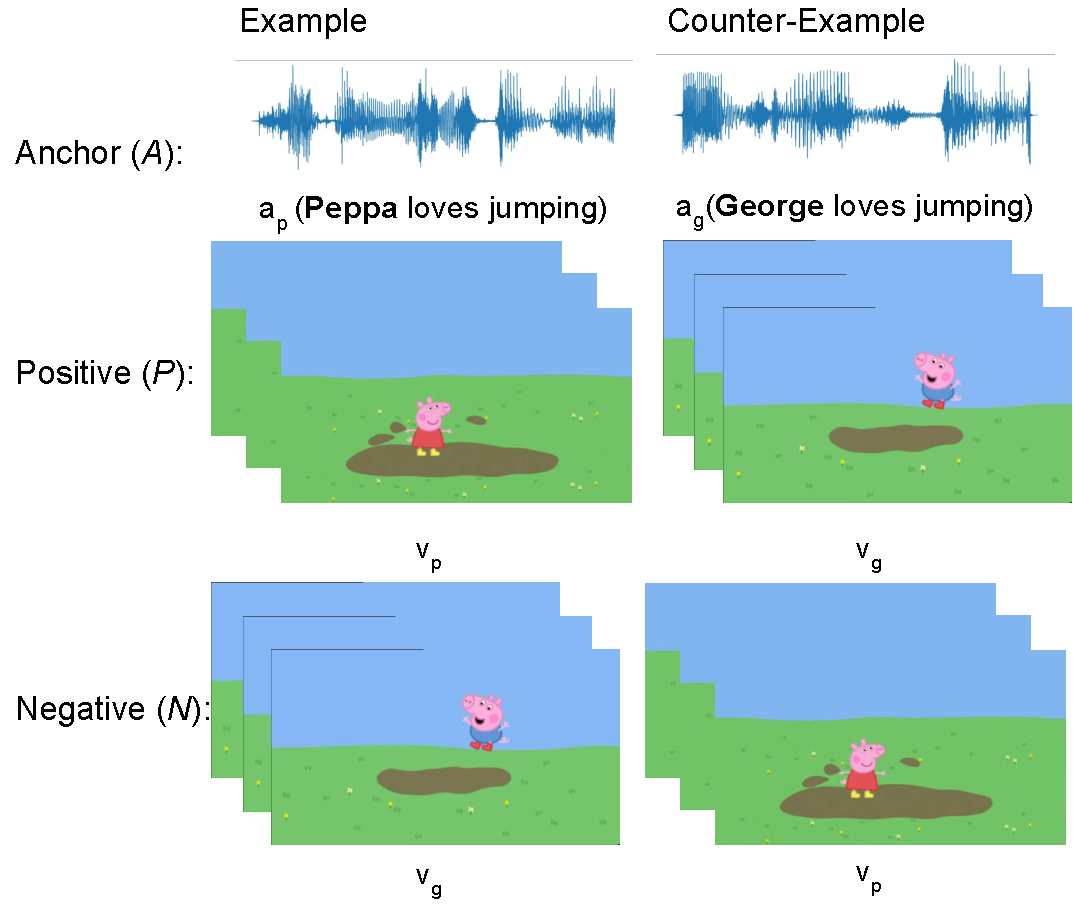
\includegraphics[width=\columnwidth]{peppa_targeted_triplets.pdf}
  \caption{Minimal Pairs Evaluation}
  \label{fig:minimal_pairs}
\end{figure}

We measure per-word accuracy by calculating the triplet accuracy (cf. 
\Cref{eq:triplet-acc}) for all triplets that contain a given word (e.g.\ 
\textit{Peppa}) either as target or distractor word, i.e.\ cases in which the 
model needs to succeed in either choosing a video
containing the given word (the example triplet in Figure
\ref{fig:minimal_pairs}) or rejecting a video containing the given
word (the counter-example triplet in Figure
\ref{fig:minimal_pairs}).
%\footnote{In this way, both the example and the counter-example shown in 
%Figure \ref{fig:minimal_pairs} are also used to assess the acquisition of the 
%word ``George''.} 
We report accuracy for all words (nouns and verbs) for which we find at least 
100 pairs of triplets.\footnote{We did not find enough examples for any 
adjectives in the data to perform an evaluation on them.}



\section{Experimental Settings}
We implement the architecture in PyTorch \citep{NEURIPS2019_9015}. We
use the Adam optimizer \citep{kingma2014adam} with the scheduling
described in \citep{devlin-etal-2019-bert}. We train every
configuration on a single GPU and stop training after 48 hours, with
batch-size 8 and accumulating gradients over 8 batches, in 16 bit
precision mode. For each model configuration we save model weights
after each epoch and report results for the checkpoint which gets the
best triplet accuracy on the narration validation data.
Our code is publicly available at \url{github.com/gchrupala/peppa},
and can be consulted for further details of the experimental setup.
\todo{Anonymity violation (for the final submission).}
